\section{Experimental Illustration}
\label{sec:experimental}

\textbf{Testbed and dataset.} We evaluate \ARES{} on
\SAFK{}, a labelled corpus of $1{,}000$ agent execution traces produced by
the \ARESBench{} testbed under controlled mismatch injection. The corpus
contains $1{,}000$ executions in total: $750$ LLM-agent executions
(Mistral-7B-Instruct backbone) and $250$ rule-based control executions.
It spans four agent architectures (a single-agent LangGraph ReAct loop, a
three-stage AutoGen pipeline, a role-based CrewAI crew, and a rule-based
Sigma/YARA control) and five threat classes (Ransomware, Phishing, Insider
Threat, DDoS, APT Intrusion), with $250$ traces per architecture. Each trace records the task requirements
$\langle\Sk^*,\K^*,\CC^*\rangle$, the injected mismatch levels
$\delta_S,\delta_K,\delta_C \in \{0,\tfrac{1}{3},\tfrac{2}{3},1\}$, the
agent output, the agent's stated confidence, the failure label assigned by
the labelling pipeline, and the observed reliability outcome.
The corpus is split $600/200/200$ for training, validation, and held-out
test (stratified by task class and architecture).

\textbf{Labelling protocol.} Failure modes are first assigned by a
deterministic rule-based engine that compares each agent output against
the ATT\&CK-derived ground truth using a fixed codebook. We label five
manifestations: \textit{Hallucination} (output asserts facts that
contradict or are absent from the ground-truth incident),
\textit{Omission} (a required step is silently skipped),
\textit{Paralysis} (the agent halts because a required capability is
unavailable), \textit{Confabulation} (intermediate reasoning invents
nonexistent intermediate facts), and \textit{Overclaiming} (the agent
asserts coverage of TTPs or IOCs not present in the incident). A $10\%$
stratified sample ($n = 100$) is independently reviewed by two annotators;
inter-rater agreement is Cohen's $\kappa = 0.84$ for origin code and
$\kappa = 0.91$ for manifestation code, with disagreements resolved by
adjudication and rule-based labels revised to match human judgement in
$4.3\%$ of reviewed cases.

\subsection{Knowledge Mismatch Predicts Hallucination}

Across 750 LLM-based executions, hallucination rate increases monotonically
with $\delta_K$: from 1.4\% at $\delta_K = 0$ to 39.1\% at $\delta_K = 1.0$
(Fig.~\ref{fig:e1_isaia}). The Pearson correlation is $\rho = 0.92$
($p < 0.001$), strongly supporting Hypothesis~\ref{hyp:hallucination}. The
rule-based baseline exhibits zero hallucinations regardless of $\delta_K$,
confirming hallucination as an LLM-specific failure mode.

\begin{figure}[t]
\centering
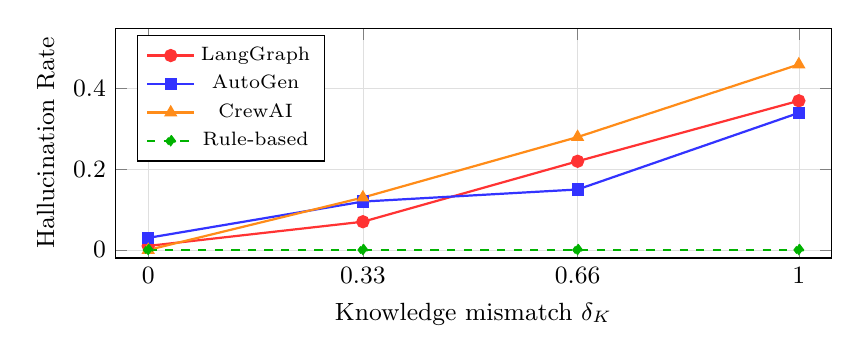
\begin{tikzpicture}
\begin{axis}[
  width=0.88\columnwidth, height=4.5cm,
  xlabel={Knowledge mismatch $\delta_K$},
  ylabel={Hallucination Rate},
  xmin=-0.05, xmax=1.05, ymin=-0.02, ymax=0.55,
  xtick={0,0.33,0.66,1.0},
  legend pos=north west,
  legend style={font=\scriptsize},
  grid=both, grid style={line width=0.2pt, draw=gray!25},
  tick label style={font=\small}, label style={font=\small},
]
\addplot[thick, color=red!80, mark=*, mark size=2]
  coordinates {(0,0.01)(0.33,0.07)(0.66,0.22)(1.0,0.37)};
\addlegendentry{LangGraph}
\addplot[thick, color=blue!80, mark=square*, mark size=1.8]
  coordinates {(0,0.03)(0.33,0.12)(0.66,0.15)(1.0,0.34)};
\addlegendentry{AutoGen}
\addplot[thick, color=orange!90, mark=triangle*, mark size=2]
  coordinates {(0,0.00)(0.33,0.13)(0.66,0.28)(1.0,0.46)};
\addlegendentry{CrewAI}
\addplot[thick, color=green!70!black, mark=diamond*, mark size=2, dashed]
  coordinates {(0,0.0)(0.33,0.0)(0.66,0.0)(1.0,0.0)};
\addlegendentry{Rule-based}
\end{axis}
\end{tikzpicture}
\caption{Hallucination Rate vs.\ knowledge mismatch $\delta_K$ across
four agent architectures ($n = 750$ LLM executions).}
\label{fig:e1_isaia}
\end{figure}

\subsection{Framework-Level Results}

We summarise four additional framework-level results.

\textbf{ARS threshold generalisation.} The optimal ARS threshold
($\theta^* = 0.58$), learned via isotonic regression on the training
split, achieves test F1 $= 0.96$ (precision $1.00$, recall $0.92$)
with the minimum per-class test F1 at $0.91$ and a one-point
train--test gap. A stricter leave-one-threat-class-out protocol
recovers mean test F1 $= 0.957$, supporting ARS as a generalisable
reliability signal rather than a class-memorising score.
The reported threshold result uses the post-execution ARS including
$\delta_R$; $\ARS^{\mathrm{pre}}$ is intended for pre-execution
screening and showed the same directional trend but lower absolute
discrimination because reasoning mismatch is unavailable before
execution.

\textbf{Distinct failure signatures per mismatch dimension.} Isolating
each mismatch dimension at $\delta = 0.66$ yields diagnostically
separable manifestation distributions (chi-square $= 146.7$,
$p < 0.001$, dof $= 18$): capability deprivation predominantly
produces Paralysis ($76\%$), skill deficit produces silent
Omission ($60\%$), and reasoning perturbation produces
Confabulation plus Overclaiming ($77\%$ combined) -- the most
dangerous signature because confidence-inflated errors are the most
likely to mislead downstream consumers.

\textbf{Cascade degradation.} The naive head-line gap between AUT-1
(single-agent LangGraph) and AUT-2 (three-stage AutoGen pipeline) is
$\sim 5.7\%$ relative ARS (mean ARS $0.659$ vs.\ $0.621$), but this
conflates framework identity with pipeline depth. A controlled
ablation on $27$ strictly matched mismatch buckets isolates the two
contributions: framework identity contributes $\mathbf{0.13\%}$
(essentially zero) and pure pipeline depth contributes
$\mathbf{17.25\%}$. The pipeline-depth effect is consistent across
all five threat classes and empirically supports
Theorem~\ref{thm:cascade} in the tightly-coupled regime, where the
empirical $\mu^*_{\max} \geq 0.8$ in $100\%$ of AUT-2 records.

\textbf{Epistemic Gap as interpretable decomposition.} Epistemic Gap
and raw knowledge mismatch achieve statistically indistinguishable
correlation with false-negative severity
($\rho_\mathcal{E} = 0.80$ vs.\ $\rho_{\delta_K} = 0.80$, Fisher
$z$-test $p = 0.78$). The value of $\mathcal{E}$ is decomposing risk
into a knowledge term ($\delta_K$) and a calibration term ($1 - U$),
exposing two independently mitigable axes. A 30-incident validation
against the live CISA KEV catalogue (post-training-cutoff, so
$\delta_K \approx 1$) yields an operational $\E$ gap of $\sim 66\%$
at matched $\delta_K$ across five frontier LLM backbones.

\textbf{Cross-model-family generalisation.} The
hallucination-versus-$\delta_K$ relationship replicates directionally
across four LLM families from 7B (Mistral-7B-Instruct) to frontier
scale (GPT-4o-mini, Claude Haiku~4.5, Claude Sonnet~4.6), with
bucket-aggregated $\rho \in [0.78, 0.95]$; absolute thresholds require
per-model recalibration.

Together with the knowledge-hallucination relationship in
Fig.~\ref{fig:e1_isaia}, these results indicate that \ARES{} captures
meaningful, generalisable reliability signals across diverse agent
architectures and threat scenarios.
